\ofsubsection{Bestiário}
%
\ofquote{"Ao longo do tempo, o mundo encontra maneiras novas e empolgantes de matar um homem."}{Balthier}
%
\\\\
%

\includegraphics[width=\columnwidth]{./art/images/ff6.jpg}
%
\vfill
%
\accf{Encontros de combate} podem ocorrer em várias situações diferentes, como por exemplo, o grupo tenta fugir de uma gangue de bandidos ou terão que enfrentar o grande vilão num confronto épico.
O combate é geralmente uma questão de vida ou morte e pode tomar uma parte significante do tempo de jogo. 
No entanto, nem sempre tem que ser uma luta até a morte, pois o grupo pode tentar soluções alternativas, como negociar ou escapar. 
Durante o combate, o MJ representa o papel de todos os adversários, aplicando as regras de combate a eles, embora possa manter informações cruciais secretas, como atributos e rolagens de dados dos inimigos.
Enquanto jogando como um grupo inimigo, tente tomar decisões da perspectiva deles, sem usar seu próprio conhecimento.
Além disso, também é útil usar auxílio visual, como mapas, a fim de acompanhar o desenvolver no campo de batalha.
As \accf{Recompensas de combate} normalmente fazem uma grande parte da riqueza do grupo e a tabela abaixo oferece orientações aproximadas a depender do nível do grupo.
Um grupo com Gil insuficiente não pode pagar por itens essenciais, mas aquele com bastante, pode evitar muitas consequências.
As recompensas nem sempre são em Gil, podem ser equipamentos, itens ou materiais de valor parecido e por padrão, são divididos entre todos os membros do grupo.
%
\vfill
%
\oftable{p{0.3\columnwidth} p{0.7\columnwidth}}
{\accf{Nível} & \accf{Recompensa de combate por jogador}}
{
	1 & 200G \ofrow
	2 & 300G \ofrow
	3 & 500G \ofrow
	4 & 800G \ofrow
	5 & 1.000G \ofrow
	6 & 1.200G \ofrow
	7 & 1.500G \ofrow
	8 & 2.000G \ofrow
	9 & 2.500G \ofrow
	10 & 3.000G
}
%
\newpage
%
A dificuldade dos encontros de combate variam muito e você pode adequá-los a depender do contexto e das preferências de seu grupo.
Por outro lado, o combate é a causa mais comum da morte de personagens, então se recomenda cuidado a fim de evitar surpresas inesperadas.
Mesmo assim, normalmente é desejável que o combate seja um desafio considerável.
Alcançar um equilíbrio satisfatório pode exigir algum esforço, porque a dificuldade do encontro depende de vários fatores:
Primeiro, as circunstancias da batalha podem afetar consideravelmente esse equilíbrio.
Como por exemplo, os jogadores estarão em grande desvantagem ao já terem sidos afetados por batalhas anteriores no mesmo dia ou quando o grupo adversários consegue uma rodada surpresa.
Além do mais, a composição e preparação de ambos os grupos afetam bastante o resultado.
Como por exemplo, um grupo de apenas lutadores físicos não terão problemas com inimigos comuns, o que pode não se repetir com inimigos que atacam à distância e aplicam Efeitos de estado.
Por fim, a experiência de sue grupo também terão grande impacto.
Como por exemplo, os jogadores novatos podem perder oportunidades, enquanto aqueles com muita experiência frequentemente sacam truques de suas mangas.
Contudo, infelizmente não é possível determinar as regras que se aplicam a cada grupo e situação.
Mesmo assim, pode-se discutir algumas orientações aproximadas e regras de ouro que podem ser consideradas.
Note que geralmente erramos pela precaução, com conselhos e conteúdo preparado, e você é encorajado a modificá-los em caso de não servirem adequadamente. 
%
\ofpar
%
Ao montar um grupo inimigo, recomenda-se ter um números de integrantes similar ao grupo dos jogadores e em que a força deles seja parecida.
Grandes hordas de inimigos fracos provavelmente vão sobrepujar o grupo, enquanto aqueles solitários, raramente terão alguma chance.
Uma configuração equilibrada garante que dois recursos importantes sejam parecidos: o número e força das ações de combate de ambos os lados.
Para medira a força de um inimigo, use Níveis que podem ser comparados aos dos jogadores.
Como por exemplo, se um grupo tem 4 personagens, o grupo adversário deve conter a mesma quantidade e nível.
o próximo passo é usar as seguintes orientações para determinar seus atributos:
Para cada nível, o inimigo ganha 6 \accf{Pontos de atributo}, dos quais cada ponto são iguais ao PV/PM~+5 ou FOR/MAG/DEF/RES~+1.
A AGI deles dever variar de 1 e 4, do contrário ataques comuns serão inefetivos.
Assim como os personagens, os inimigos podem usar Magias e Técnicas, além de habilidades Passivas e de Reação.
No entanto, recomenda-se manter a quantidade de habilidades inimigas baixa a fim de permitir decisões rápidas em combate.
Embora, sinta-se livre para lhes dar acesso a habilidades únicas ou exóticas.
Considere qualquer equipamento nos atributos totais de um inimigo e para armas, atribua o Dano do nível de equipamento de acordo com o nível dele.
Você também pode adicionar mais profundidade aos inimigos ao atribuir resistências e fraquezas elementais ou imunidades a estados de efeito.
Durante o combate, você pode dar dicas sutis sobre estas especialidades aos jogadores, ao narrar as ações de combate e seus efeitos.
%
\vfill
%
Em alguns casos, pode ser mais interessante criar um grupo adversário que é desbalanceado em número.
Como por exemplo, você pode querer que o grupo enfrente uma horda de inimigos fracos ou um único inimigo forte, o tal \accf{Chefe}.
Portanto, nesses casos, a força dos inimigos será diferente das dos jogadores.
No caso do grupo de inimigos superam em número o dos jogadores, recomenda-se usar inimigos de níveis mais baixo em que a soma de todos os níveis se igualem ou se aproximem em ambos os grupos.
No caso do inimigo ser superado em número, eles precisam de mais força para lidar com vários adversários.
Além de atributos aumentados, \accf{Características de chefe} podem ajudar aos seus Chefes a compensar a falta de aliados.
Características de chefe são habilidades especiais particularmente fortes, que garantem aos inimigos ações adicionais e durabilidade.
Recomenda-se as seguintes orientações para equilibrar um chefe: para cada adversário extra com que ele é capaz de lidar, dê 2 Pontos de atributo extras por nível assim como uma característica de chefe.
Como por exemplo, um chefe de Nível 5, lutando contra um grupo de 4 personagens devem ter pelo menos \mbox{5 x (6 + 3 x 2) = 60 Pontos de atributo} e 3 características de chefe.
Uma lista delas está ao lado.
%
\vfill
%
Os seguintes tipos de configuração de grupo de inimigos irregularmente equilibrados são usadas normalmente:
\ofrow
\accf{Chefe único:}
Um inimigo poderoso sozinho, pode ser um exemplo do vilão principal.
Ue as orientações mencionadas acima para garantir que o chefe pode lidar com muitos jogadores.
Um chefe único também se beneficia bastante de especialidades extras, tais quais interações especiais com o ambiente.
Esta variante é o equilíbrio mais complicado, então é recomendado outras sempre que possível.
\ofrow
\accf{Conselho de chefes:} 
O grupo de inimigos consistem de pequeno grupo de Chefes, geralmente de 2 a 3 com cada um sendo equivalente em força, mas mais forte do que um personagem.
Normalmente,suas forças se complementam, por exemplo, um Chefe pode se forcar na ofensiva enquanto os outros se destacam em cura.
\ofrow
\accf{Chefe com lacaios:} 
Este chefe tem vários inimigos comuns trabalhando com eles, por exemplo, um Necromante levantando sua horda de mortos-vivos.
Neste caso, o chefe é mais forte do que o jogador enquanto que os lacaios, mas fracos.
\ofrow
\accf{Chefe múltiplas-partes:} 
Este tipo de chefe é representado por várias partes.
Cada parte é construída como um inimigo com seu próprio turno, atributos e habilidades, mas todas elas só podem se mover em conjunto uma vez.
Geralmente, uma das partes age como o núcleo, ao morrer, todas as outras morrem com ela.
É comum que o núcleo também tenha proteção extra e a habilidade de regenerar outras partes que tenham sofrido de KO.
\ofrow
\accf{horda inimiga:} 
Um grande grupo de inimigos comuns, geralmente do mesmo tipo e de nível menor do que os jogadores.
No entanto, aconselha-se contra um grupo que supere os jogadores em 2 para 1, por exemplo, se tiver 4 deles, eles não devem enfrentar mais do que 8 inimigos de uma vez.
%
\newpage
%
\oftable{p{0.24\columnwidth} p{0.7\columnwidth}}
{\accf{Características de Chefe} & \accf{Efeito}}
{
	Auto-Acerto & Ataque acertam sempre, mas não geram Críticos. \ofrow
	Auto-Oscilar & Permanentemente Oscilando. \ofrow
	Auto-Acelerar & Permanentemente Acelerado. \ofrow
	Auto-Regenerar & Permanentemente Regenerando. \ofrow
	Auto-Apressar & tenha 2 turnos por rodada. \ofrow
	Superimune & Imunidade permanente a todos os Estados de efeito negativos. \ofrow
	Revidar & Uma vez por rodada, ao sofrer dano, pode atacar o agressor, se ele estiver ao alcance. \ofrow
	TC-0 & O tempo de conjuração de magias e técnicas é 0r.\ofrow
	Golpe duplo & Com cada ataque, pode alvejar 2 alvos diferentes ao alcance. \ofrow
	Desvanecer & Pode se evadir de magias assim como de ataques. \ofrow
	Ataque final & Quando sofrer KO, pode agir antes de cair inconsciente. \ofrow
	Reverter & Uma vez por rodada, pode repetir a rolagem de um dado após a rolagem. \ofrow 
	Retaliar & Uma vez por rodada, ao sofrer dano, pode usar uma habilidade contra o agressor ao alcance. \ofrow
	Surtar & Ao ter PV reduzido abaixo da metade, ganhe AuFOR, AuDEF, AuMAG e AuRES até o fim da batalha. \ofrow
}
%
\vfill
%
\accf{Gladio: "Então, este espadachim..." \\ Cor: "Ele é um mestre das lâminas. Ahm, esperava algo mais profundo?"}
%
\vfill
%
Diferente dos jogadores, os \accf{Monstros} são outro tipo comum de adversários que o grupo enfrentam em combate.
Eles são seres selvagens que vivem em seu habitat natural, ao contato com o grupo é comum se sentirem ameaçados e atacar.
Monstros diferentes, com frequência, trabalham contra hostis e o grupo pode cruzar com alguns inteligentes, que possuem objetivos complexos.
Em geral são parte ou causa de um grande conflito e por isso, sua aventura pode ter vários monstros na trama principal.
Comparado aos personagens, eles também podem variar bastante em tamanho e aparência.
Eles são classificados como Médio~(\accf{M}), se tiverem cerca de 1u de diâmetro, Grande~(\accf{G}), se tiverem mais do que 2u e Pequeno~(\accf{P}), se tiverem menos do que 0.5u. Monstros não usam armas e armaduras comuns, mas eles têm partes similares integradas aos seus corpos, que seguem as mesmas regras.
As páginas seguintes incluem vários monstros de níveis diferentes preparados. Você deve usá-los como apresentado, mas também é encorajado a se modificar cada um deles a fim de se ajustar à necessidade ou use os como exemplos para criar os seus próprios.
%
\clearpage
%
%
%
%%%%%%%%%%%%%%%%%%%%%%%%%%%%%%%L1%%%%%%%%%%%%%%%%%%%%%%%%%%%%%%%%%%%%%%%%%
%
\ofmonster{Goblin}{1}{
\includegraphics[width=0.2\columnwidth]{./art/monsters/goblin.jpg}}
{
	PV: & \hfill 12 & PM: & \hfill 0\\
	FOR: & \hfill 2 & DEF: & \hfill 1 \\
	MAG: & \hfill 0 & RES: & \hfill 1 \\
	AGI: & \hfill 3 & Tamanho: & \hfill M\\
}
{\accf{Faca}: 1d Dano \hfill \accf{Imune}:\immobile}
{}
%
\vfill
%
\ofmonster{Esqueleto}{1}{
\includegraphics[width=0.17\columnwidth]{./art/monsters/skeleton.jpg}}
{
	PV: & \hfill 11 & PM: & \hfill 0\\
	FOR: & \hfill 2 & DEF: & \hfill 2 \\
	MAG: & \hfill 0 & RES: & \hfill 0 \\
	AGI: & \hfill 2 & Tamanho: & \hfill M \\   
}
{\accf{Espada}: 1d Dano \hfill \accf{Fraco}:\fire\holy}
{\mpassive{Morto-vivo}{Zumbi permanentemente.}}
%
\vfill
%
\ofmonster{Mandrágora}{1}{
\includegraphics[width=0.14\columnwidth]{./art/monsters/mandragora.jpg}}
{
	PV: & \hfill 10 & PM: & \hfill 18\\
	FOR: & \hfill 0 & DEF: & \hfill 0 \\
	MAG: & \hfill 0 & RES: & \hfill 1 \\
	AGI: & \hfill 2 & Tamanho: & \hfill P\\
}
{\accf{Cabeçada}: 1d Dano \hfill \accf{Fraco}:\lightning}
{\mspell{Dormir}{6}{0r}{Único}{3u}{O alvo faz um teste de DC 8 ou fica Adormecido por 43 rodadas.}{\sleep}}
%
\vfill
%
\ofmonster{Tarântula}{1}{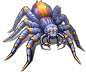
\includegraphics[width=0.25\columnwidth]{./art/monsters/tarantula.jpg}}
{
	PV: & \hfill 10 & PM: & \hfill 16\\
	FOR: & \hfill 1 & DEF: & \hfill 0 \\
	MAG: & \hfill 0 & RES: & \hfill 0 \\
	AGI: & \hfill 3 & Tamanho: & \hfill P\\
}
{\accf{Mordida}: 1d Dano \hfill \accf{Fraco}:\fire \hfill \accf{Imune}:\poison}
{\mtech{Teia}{4}{0r}{Único}{5u}{O alvo faz um teste de DC 8 ou fica Imóvel por 1 rodada.}{\immobile}}	
%
\vfill
%
\ofmonster{Bandersnatch}{1}{
\includegraphics[width=0.27\columnwidth]{./art/monsters/bandersnatch.jpg}}
{
	PV: & \hfill 10 & PM: & \hfill 6\\
	FOR: & \hfill 2 & DEF: & \hfill 1 \\
	MAG: & \hfill 0 & RES: & \hfill 0 \\
	AGI: & \hfill 3 & Tamanho: & \hfill M\\
}
{\accf{Garra}: 1d Dano \hfill \accf{Fraco}:\ice}
{\mtech{Mordida}{2}{0r}{Único}{1u}{Ataque o alvo, se acertar, cause dano e ignore a DEF dele.}{}}	
%
\vfill 
%
%%%%%%%%%%%%%%%%%%%%%%%%%%%%%%%L2%%%%%%%%%%%%%%%%%%%%%%%%%%%%%%%%%%%%%%%%%
%
%
\ofmonster{Sahagin}{2}{
\includegraphics[width=0.17\columnwidth]{./art/monsters/sahagin.jpg}}
{
	PV: & \hfill 16 & PM: & \hfill 24\\
	FOR: & \hfill 1 & DEF: & \hfill 0 \\
	MAG: & \hfill 2 & RES: & \hfill 1 \\
	AGI: & \hfill 3 & Tamanho: & \hfill M\\
}
{\accf{Lança}: 1d Dano \hfill \accf{Resistente}:\water \hfill \accf{Fraco}:\lightning}
{\mspell{Água}{6}{0r}{Único}{4u}{Cause 2d de dano de Água ao alvo.}{\water}}
%
\newpage
%
\ofmonster{Basilisco}{2}{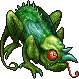
\includegraphics[width=0.2\columnwidth]{./art/monsters/basilisk.jpg}}
{
	PV: & \hfill 17 & PM: & \hfill 16 \\
	FOR: & \hfill 2 & DEF: & \hfill 2 \\
	MAG: & \hfill 0 & RES: & \hfill 1 \\
	AGI: & \hfill 3 & Tamanho: & \hfill M\\
}
{\accf{Lambida}: 1d Dano \hfill \accf{Resistente}:\earth \hfill \accf{Fraco:}\water}
{\mpassive{Toque de pedra}{Ao acertar um ataque, o alvo faz um teste de DC 7 ou fica Imóvel por 3 rodada.}}
%
\vfill
%
\ofmonster{Carniçal}{2}{
\includegraphics[width=0.18\columnwidth]{./art/monsters/ghoul.jpg}}
{
	PV: & \hfill 18 & PM: & \hfill 20\\
	FOR: & \hfill 2 & DEF: & \hfill 1 \\
	MAG: & \hfill 1 & RES: & \hfill 2 \\
	AGI: & \hfill 2 & Tamanho: & \hfill M\\
}
{\accf{Garra}: 1d Dano \hfill \accf{Fraco}:\fire\holy \hfill \accf{Resistente}:\ice}
{	
	\mtech{Modida zumbi}{3}{0r}{Única}{1u}{O alvo recebe 1d de dano e faz um teste de DC 8, se falhar, fica Zumbi por 5 rodadas.}{\zombie}		
	\mpassive{Morto-vivo}{Zumbi permanentemente.}
}
%
\vfill
%
\ofmonster{Cocatriz}{2}{
\includegraphics[width=0.2\columnwidth]{./art/monsters/cockatrice.jpg}}
{
	PV: & \hfill 15 & PM: & \hfill 16\\
	FOR: & \hfill 3 & DEF: & \hfill 1 \\
	MAG: & \hfill 0 & RES: & \hfill 2 \\
	AGI: & \hfill 3 & Tamanho: & \hfill M\\
}
{\accf{Bico}: 1d Dano \hfill \accf{Fraco}:\lightning}
{\mspell{Cegar}{6}{0r}{Único}{3u}{O alvo faz um teste de DC 8 ou fica Cego por 3 rodadas.}{\blind}}
%
\vfill
%
\ofmonster{Coeurl}{2}{
\includegraphics[width=0.23\columnwidth]{./art/monsters/coeurl.jpg}}
{
	PV: & \hfill 20 & PM: & \hfill 15\\
	FOR: & \hfill 2 & DEF: & \hfill 1 \\
	MAG: & \hfill 0 & RES: & \hfill 2 \\
	AGI: & \hfill 3 & Tamanho: & \hfill M\\
}
{\accf{Garra}: 1d Dano}
{\mtech{Raio d energia}{5}{0r}{Único}{5u}{O alvo faz um teste de DC 8 ou fica Imóvel por 3 rodadas.}{\immobile}}
%
\vfill
%
%
%%%%%%%%%%%%%%%%%%%%%%%%%%%%%%%L3%%%%%%%%%%%%%%%%%%%%%%%%%%%%%%%%%%%%%%%%%
%
%
% 
\ofmonster{Arimã}{3}{
\includegraphics[width=0.25\columnwidth]{./art/monsters/ahriman.jpg}}
{
	PV: & \hfill 20 & PM: & \hfill 24\\
	FOR: & \hfill 2 & DEF: & \hfill 1 \\
	MAG: & \hfill 0 & RES: & \hfill 4 \\
	AGI: & \hfill 4 & Tamanho: & \hfill P\\
}
{\accf{Feixe}: 1d Dano, 3u Alcance}
{\mtech{Onda de choque sinistra}{6}{0r}{Única}{3u}{O alvo faz um teste de DC 8 ou sofre 2d de dano e fica Mudo por 3 rodadas.}{\silence}}
%
\clearpage
%
\ofmonster{Abelha assassina}{3}{
\includegraphics[width=0.17\columnwidth]{./art/monsters/killerbee.jpg}}
{
	PV: & \hfill 20 & PM: & \hfill 18 \\
	FOR: & \hfill 3 & DEF: & \hfill 1 \\
	MAG: & \hfill 0 & RES: & \hfill 3 \\
	AGI: & \hfill 3 & Tamanho: & \hfill P\\
}
{\accf{Ferrão}: 1d Dano \hfill \accf{Imune}:\poison}
{\mpassive{Veneno}{Cada alvo que rolar abaixo de 6 ao se evadir contra seu ataque, fica Envenenado por 3 rodadas.}}
%
\vfill
%
\ofmonster{Pudim azul}{3}{
\includegraphics[width=0.3\columnwidth]{./art/monsters/flan.jpg}}
{
	PV: & \hfill 15 & PM: & \hfill 30\\
	FOR: & \hfill 0 & DEF: & \hfill 4 \\
	MAG: & \hfill 5 & RES: & \hfill 1 \\
	AGI: & \hfill 1 & Tamanho: & \hfill M\\
}
{\accf{Pancada}: 1d Dano \hfill \accf{Resistente}:\ice \hfill \accf{Fraco}:\fire }
{\mspell{Nevasca}{4}{0r}{Único}{3u}{Cause 2d de dano de Gelo ao alvo. }{\ice}}
%
\vfill
%
\ofmonster{Bomba}{3}{
\includegraphics[width=0.23\columnwidth]{./art/monsters/bomb.jpg}}
{
	PV: & \hfill 25 & PM: & \hfill 15\\
	FOR: & \hfill 3 & DEF: & \hfill 2 \\
	MAG: & \hfill 2 & RES: & \hfill 1 \\
	AGI: & \hfill 3 & Tamanho: & \hfill M\\
}
{\textbf{Pancada}: 1d Dano \hfill \textbf{Resistente}:\fire \hfill \textbf{Fraco}:\ice }
%{}
{\mtech{Auto-Destruição}{15}{1r}{2u}{Você}{Cause KO em si mesmo para causar 4d de dano de fogo a todos dentro da área.}{\fire}}
%
%\ofmonster{Death Claw}{3}{
\includegraphics[width=0.25\columnwidth]{./art/monsters/deathclaw.jpg}}
%{
%	HP: & \hfill 26 & MP: & \hfill 15\\
%	STR: & \hfill 2 & DEF: & \hfill 2 \\
%	MAG: & \hfill 0 & RES: & \hfill 1 \\
%	AGI: & \hfill 3 & Size: & \hfill M\\
%}
%{\accf{Claw}: 1d DMG}
%{\mtech{Grapple}{5}{0r}{Single}{2u}{The target becomes grappled and at the start of each turn he can make a DC~8 check to free himself. While grappled, the target suffers Immobile and an additional 1d damage for each failed attempt to free himself.}{}}
%
\vfill
%
\ofmonster{Feiticeiro}{3}{
\includegraphics[width=0.23\columnwidth]{./art/monsters/sorcerer.jpg}}
{
	PV: & \hfill 25 & PM: & \hfill 50\\
	FOR: & \hfill 0 & DEF: & \hfill 1 \\
	MAG: & \hfill 3 & RES: & \hfill 2 \\
	AGI: & \hfill 2 & Tamanho: & \hfill M\\
}
{\accf{Raio de energia}: 1d Dano, 3u Alcance \hfill \accf{Imune:}\silence\demag}
{
	\mspell{Silêncio}{6}{0r}{Único}{5u}{O alvo faz um teste de DC 8 ou fica Mudo por 3 rodadas.}{}
	\mspell{drenar}{8}{0r}{Único}{4u}{Reduz o PV do alvo em 1d e aumente o seu na mesma quantidade.}{}
}
%
\vfill
%
%%%%%%%%%%%%%%%%%%%%%%%%%%%%%%%L4%%%%%%%%%%%%%%%%%%%%%%%%%%%%%%%%%%%%%%%%%
%
%
\ofmonster{Formiga-leão}{4}{
\includegraphics[width=0.28\columnwidth]{./art/monsters/antlion.jpg}}
{
	PV: & \hfill 45 & PM: & \hfill 24\\
	FOR: & \hfill 2 & DEF: & \hfill 3 \\
	MAG: & \hfill 0 & RES: & \hfill 1 \\
	AGI: & \hfill 3 & Tamanho: & \hfill M\\
}
{\accf{Mordida}: 2d Dano \hfill \accf{Resistente}:\earth}
{\mtech{Tempestade de areia}{8}{0r}{3u}{Você}{Todos os inimigos na área sofrem 2d de dano de Terra e ficam Cegos por 1 rodada.}{\earth \blind}}
%
\newpage
%
\ofmonster{Diabrete}{4}{
\includegraphics[width=0.17\columnwidth]{./art/monsters/imp.jpg}}
{
	PV: & \hfill 30 & PM: & \hfill 40 \\
	FOR: & \hfill 2 & DEF: & \hfill 1 \\
	MAG: & \hfill 5 & RES: & \hfill 4 \\
	AGI: & \hfill 4 & Tamanho: & \hfill P\\
}
{\accf{Garra}: 2d Dano \hfill \accf{Imune:}\sleep \hfill \accf{Resistente}:\dark}
{	
	\mspell{Confusão}{10}{0r}{Único}{5u}{
		O alvo faz um teste de DC 8 ou você toma o seu controle no próximo turno dele. 
		Comende-o a se mover e atacar qualquer alvo à sua escolha, incluindo a si mesmo.
	}{}	
}
%
\vfill
%
\ofmonster{Minotauro}{4}{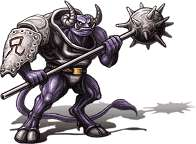
\includegraphics[width=0.3\columnwidth]{./art/monsters/minotaur.jpg}}
{
	PV: & \hfill 40 & PM: & \hfill 24 \\
	FOR: & \hfill 3 & DEF: & \hfill 2 \\
	MAG: & \hfill 0 & RES: & \hfill 1\\
	AGI: & \hfill 2 & Tamanho: & \hfill M\\
}
{\accf{Mangual}: 2d Dano \hfill \accf{Resistente}:\earth\fire}
{
	\mtech{Quebra-chão}{6}{0r}{3u (linha)}{Você}{Todos na área sofrem 3d de dano de Terra. }{\earth}	
	\mreaction{Reforçar}{Enquanto seu PV estiver abaixo da metade, ganhe AuFOR.}
}
%
\vfill
%
\ofmonster{Fantasma}{4}{
\includegraphics[width=0.2\columnwidth]{./art/monsters/ghost.jpg}}
{
	PV: & \hfill 35 & PM: & \hfill 50 \\
	FOR: & \hfill 2 & DEF: & \hfill 1 \\
	MAG: & \hfill 0 & RES: & \hfill 0 \\
	AGI: & \hfill 2 & Tamanho: & \hfill M\\
}
{\accf{Mordida}: 2d Dano \hfill \accf{Resistente}:\fire \hfill \accf{Fraco}:\ice}
{
	\mspell{Fogo}{4}{0r}{Único}{3u}{O alfo sofre 2d de dano de Fogo.}{\fire}	
	\mpassive{Imaterial}{Danos físicos causam metade do dano.}
	\mpassive{Morto-vivo}{Zumbi permanentemente.}
}
%
\vfill
%
\ofmonster{Cavaleiro Negro}{4}{
\includegraphics[width=0.22\columnwidth]{./art/monsters/blackknight.jpg}}
{
	PV: & \hfill 90 & PM: & \hfill 50 \\
	FOR: & \hfill 5 & DEF: & \hfill 3 \\
	MAG: & \hfill 0 & RES: & \hfill 4 \\
	AGI: & \hfill 3 & Tamanho: & \hfill M\\
}
{\accf{Espada}: 2d Dano \hfill \accf{Resistente}:\dark\ice \hfill \accf{Fraco}:\holy\fire \\ \accf{Golpe duplo, Revidar} \hfill \accf{Imune}:\poison\blind}
{
	\mtech{Executar}{8}{0r}{Único}{1u}{Só pode mirar inimigos com PV até a metade. O alvo faz um teste de DC]8 ou sofre KO.}{}	
	\mtech{Escuridão}{6}{0r}{3u}{5u}{Crie um Campo obscuro na área que dura por 3 rodadas.}{}	
}
%
\clearpage
%
%%%%%%%%%%%%%%%%%%%%%%%%%%%%%%%L5%%%%%%%%%%%%%%%%%%%%%%%%%%%%%%%%%%%%%%%%%
%
%
\ofmonster{Gigas}{5}{
\includegraphics[width=0.16\columnwidth]{./art/monsters/gigas.jpg}}
{
	PV: & \hfill 80 & PM: & \hfill 60\\
	FOR: & \hfill 5 & DEF: & \hfill 4 \\
	MAG: & \hfill 0 & RES: & \hfill 3 \\
	AGI: & \hfill 1 & Tamaho: & \hfill G\\
}
{\accf{Punho}: 2d Dano, 2u Alcance \hfill \accf{Ataque final}}
{
	\mtech{Cabeçada}{8}{0r}{Único}{2u}{cause 4d de dano ao alvo e empurre-o até 3u de você.}{}
	\mtech{Terrível}{10}{0r}{3u}{Você}{inimigos na área fazem um teste de  DC~7 ou sofrem ReFOR e ReDEF por 3 rodadas.}{}
}
%
\vfill
%
\ofmonster{Wyvern}{5}{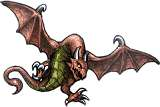
\includegraphics[width=0.29\columnwidth]{./art/monsters/wyvern.jpg}}
{
	PV: & \hfill 45 & PM: & \hfill 50 \\
	FOR: & \hfill 3 & DEF: & \hfill 3 \\
	MAG: & \hfill 3 & RES: & \hfill 2 \\
	AGI: & \hfill 3 & Tamanho: & \hfill M\\
}
{\accf{Garra}: 2d Dano \hfill \accf{Imune}:\immobile \hfill \accf{Resistente}:\wind}
{	
	\mspell{Aero}{8}{0r}{Único}{4u}{Cause 2d de dano de Vento ao alvo.}{\wind}
	\mpassive{Mergulho}{Todo alvo que rolar abaixo de 6 ao evadir-se, ele fica Imóvel por 1 rodada.}
}
%
\vfill
%
\ofmonster{Quimera}{5}{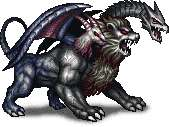
\includegraphics[width=0.3\columnwidth]{./art/monsters/chimera.jpg}}
{
	PV: & \hfill 70 & PM: & \hfill 100\\
	FOR: & \hfill 1 & DEF: & \hfill 2 \\
	MAG: & \hfill 2 & RES: & \hfill 3 \\
	AGI: & \hfill 3 & Tamanho: & \hfill M\\
}
{\accf{Garra}: 2d Dano \hfill \accf{Retaliar} \hfill \accf{Resistente}:\fire\ice\lightning}
{
	\mspell{Fogaga}{12}{1r}{Único}{5u}{Cause 6d de dano de Fogo ao alvo.}{\fire}	
	\mspell{Nevasga}{12}{1r}{Único}{5u}{Cause 6d de dano de Gelo ao alvo.}{\ice}	
	\mspell{Raiaga}{12}{1r}{Único}{5u}{Cause 6d de dano de Raio ao alvo.}{\lightning}	
}
%
\vfill
%
\ofmonster{Cacto}{5}{
\includegraphics[width=0.16\columnwidth]{./art/monsters/cactuar.jpg}}
{
	PV: & \hfill 25 & PM: & \hfill 60\\
	FOR: & \hfill 5 & DEF: & \hfill 0 \\
	MAG: & \hfill 0 & RES: & \hfill 15 \\
	AGI: & \hfill 4 & Tamanho: & \hfill P\\
}
{\accf{Pancada:} 1d Dano \hfill \accf{Auto-Oscilar}}
{	
	\mtech{1000 agulhas}{10}{0r}{Único}{1u}{Cause 10d de dano ao alvo.}{}	
	\mpassive{Fugir}{Ao fuir de inimigos, mova-se 2u além do normal.}	
}
%
\newpage
%
\ofmonster{Pote mágico}{5}{
\includegraphics[width=0.16\columnwidth]{./art/monsters/magicpot.jpg}}
{
	PV: & \hfill 1 & PM: & \hfill 0\\
	FOR: & \hfill 0 & DEF: & \hfill 99 \\
	MAG: & \hfill 0 & RES: & \hfill 99 \\
	AGI: & \hfill 1 & Tamanho: & \hfill P\\
}
{	\accf{Superimune}}
{
	\mreaction{Me dá!}{Ao receber um item benéfico, desapareça (KO) e deixe 1.000G. Ao ser atacado, faça um teste de DC 8 ou sofra KO para causar 8d de dano em 3u ao seu redor, sem deixar Gil.}
}
%
\vfill
%
%%%%%%%%%%%%%%%%%%%%%%%%%%%%%%%L6%%%%%%%%%%%%%%%%%%%%%%%%%%%%%%%%%%%%%%%%%
%
%
\ofmonster{Devorador de mentes}{6}{
\includegraphics[width=0.23\columnwidth]{./art/monsters/mindflayer.jpg}}
{
	PV: & \hfill 60 & PM: & \hfill 70 \\
	FOR: & \hfill 0 & DEF: & \hfill 3 \\
	MAG: & \hfill 5 & RES: & \hfill 4 \\
	AGI: & \hfill 2 & Tamanho: & \hfill M\\
}
{\accf{Cajado}: 1d Dano \hfill \accf{Imune}:\poison\silence\sleep \hfill \accf{Resistente}:\water}
{	
	\mspell{Aguarga}{14}{1r}{Único}{6u}{Cause 6d de dano de Água ao alvo. }{\water}
	\mtech{Onda mental}{12}{1r}{2u}{5u}{Inimigos na área sofrem 4d de dano e ficam Imóveis por 1 rodada.}{\immobile \dark}	
}
%
\vfill
%
\ofmonster{Lâmia}{6}{
\includegraphics[width=0.24\columnwidth]{./art/monsters/lamia.jpg}}
{
	PV: & \hfill 65 & PM: & \hfill 50 \\
	FOR: & \hfill 3 & DEF: & \hfill 4 \\
	MAG: & \hfill 2 & RES: & \hfill 4 \\
	AGI: & \hfill 3 & Tamanho: & \hfill M\\
}
{\accf{Bofetada}: 2d Dano\hfill \hfill \accf{Imune}:\poison\sleep\silence \hfill \accf{Fraco}:\lightning}
{	
	\mspell{Sapo}{16}{1r}{Único}{5u}{
		O alvo faz um teste de DC 8 ou é transformado em sapo por 3 rodadas ou até receber dano.
		Enquanto transformado, o alvo não pode falar ou agir e só pode se mover 1u por turno.
	}{}	
	\mreaction{Atrair}{
		Ao ser atingida com um ataque pelo inimigo, ele deve fazer um teste de DC~6 ou você pode decidir seus movimentos e ações no próximo turno dele.
	}
}
%
\vfill
%
\ofmonster{Gigante de ferro}{6}{
\includegraphics[width=0.19\columnwidth]{./art/monsters/irongiant.jpg}}
{
	PV: & \hfill 130 & PM: & \hfill 80 \\
	FOR: & \hfill 7 & DEF: & \hfill 5 \\
	MAG: & \hfill 0 & RES: & \hfill 4 \\
	AGI: & \hfill 2 & Tamanho: & \hfill G\\
}
{\accf{Espada}: 2d Dano, 2u Alcance \hfill \accf{Revidar, Surto}}
{
	\mtech{Golpe amplo}{6}{0r}{3u (frontal)}{Você}{Faça um ataque contra os inimigos na área de efeito.}{}		
	\mtech{Tremor}{12}{0r}{5u (linha)}{Você}{inimigos na área fazem um teste de DC~8 ou sofrem 2d de dano, ficam Imóveis e ganham ReDEF por 1 rodada. }{}		
}
%
\newpage
%
\ofmonster{Medusa}{6}{
\includegraphics[width=0.22\columnwidth]{./art/monsters/medusa.jpg}}
{
	PV: & \hfill 60 & PM: & \hfill 70\\
	FOR: & \hfill 3 & DEF: & \hfill 2 \\
	MAG: & \hfill 5 & RES: & \hfill 3 \\
	AGI: & \hfill 3 & Tamanho: & \hfill M\\
}
{\accf{Cabelo}: 2d Dano \hfill \accf{Imune}:\poison\sleep\immobile \hfill  \accf{Resistente}:\earth\lightning}
{	
	\mtech{Encarar}{16}{0r}{3u (frontal)}{Você}{Todos na área fazem um teste de DC~8 ou ficam Imóveis por 4 rodadas.}{\immobile}	
	\mspell{Raiaga}{12}{1r}{Único}{5u}{Cause 6d de dano de Raio ao alvo.}{\lightning}
}
%
\vfill
%
\ofmonster{Ogro}{6}{
\includegraphics[width=0.22\columnwidth]{./art/monsters/ogre.jpg}}
{
	PV: & \hfill 80 & PM: & \hfill 50 \\
	FOR: & \hfill 5 & DEF: & \hfill 3 \\
	MAG: & \hfill 0 & RES: & \hfill 2 \\
	AGI: & \hfill 2 & Tamanho: & \hfill G\\
}
{\accf{Soco}: 2d Dano, 2u Alcance \hfill \accf{Imnue}:\immobile\destr\dedef}
{	
	\mtech{Surrar}{5}{0r}{Único}{Arma}{
		Ao atacar um alvo que tenha Vantagem ao se evadir-se, se acertar, será um Acerto Crítico.
	}{}
	\mpassive{Alterar postura}{
		No fim de cada turno seu adote uma postura.
		Ofensiva: consiga um Acerto Crítico quando o alvo rolar 5 ou menos no teste de evasão. 
		Defensiva: Ao ser atingido por um ataque, você pode atacar o alvo imediatamente.
	}
}
%
\vfill
%
%
%%%%%%%%%%%%%%%%%%%%%%%%%%%%%%%L7%%%%%%%%%%%%%%%%%%%%%%%%%%%%%%%%%%%%%%%%%
%
%
\ofmonster{Cérbero}{7}{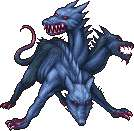
\includegraphics[width=0.23\columnwidth]{./art/monsters/cerberus.jpg}}
{
	PV: & \hfill 100 & PM: & \hfill 100 \\
	FOR: & \hfill 5 & DEF: & \hfill 3 \\
	MAG: & \hfill 3 & RES: & \hfill 4 \\
	AGI: & \hfill 3 & Tamanho: & \hfill G\\
}
{\accf{Mordida}: 2d Dano \hfill \accf{Revidar} \hfill \accf{Resistente}:\fire\ice\lightning}
{	
	\mspell{Fogaga}{12}{1r}{Único}{5u}{Cause 6d de dano de Fogo ao alvo. }{\fire}
	\mpassive{Tríade tripla}{Você pode agir contra até 3 alvos dentro do alcance ao mesmo tempo.}
}
%
\vfill
%
\ofmonster{Zu}{7}{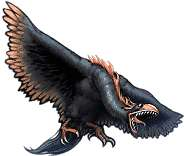
\includegraphics[width=0.25\columnwidth]{./art/monsters/zu.jpg}}
{
	PV: & \hfill 120 & PM: & \hfill 60 \\
	FOR: & \hfill 7 & DEF: & \hfill 5 \\
	MAG: & \hfill 0 & RES: & \hfill 7 \\
	AGI: & \hfill 2 & Tamanho: & \hfill G\\
}
{\accf{Bico}: 2d Dano \hfill \accf{Auto-Regenerar} \hfill \accf{Imune}:\poison\sleep\silence}
{
	\mtech{Tornado}{10}{1r}{9u (linha)}{Você}{
		Crie um tornado com 2u de diâmeto que avança 3u em linha por rodada pelas próximas 3 rodadas. 
		Qualquer um, exceto você, que entra em contato com ele, sofre 4d de dano de Vento e fica Imóvel por 1 rodada.
	}{\wind \immobile}	
}
%
\newpage
%
\ofmonster{Verme da areia}{7}{
\includegraphics[width=0.24\columnwidth]{./art/monsters/abyssworm.jpg}}
{
	PV: & \hfill 105 & PM: & \hfill 110 \\
	FOR: & \hfill 5 & DEF: & \hfill 3 \\
	MAG: & \hfill 2 & RES: & \hfill 6 \\
	AGI: & \hfill 1 & Tamanho: & \hfill G\\
}
{\accf{Ácido}: 2d Dano, 5u Alcance \hfill \accf{Resistente:}\earth\wind \hfill \accf{Golpe duplo}}
{	
	\mspell{Estremçer}{18}{1r}{3u}{10u}{Cause 6d+5 de dano de Terra a todos na área.}{\earth}
	\mtech{Inalar}{10}{0r}{Único}{3u}{você inala o alvo, removendo-o da batalha. No inicio de cada turno, ele pode tentar se livrar ao superar um teste de DC 9.}{}		
}
%
\vfill
%
\ofmonster{Malboro}{7}{
\includegraphics[width=0.24\columnwidth]{./art/monsters/malboro.jpg}}
{
	PV: & \hfill 140 & PM: & \hfill 125 \\
	FOR: & \hfill 6 & DEF: & \hfill 4 \\
	MAG: & \hfill 0 & RES: & \hfill 7 \\
	AGI: & \hfill 2 & Tamanho: & \hfill G\\
}
{
	\accf{Tentáculo}: 2d Dano \hfill \accf{Superimune, Golpe duplo}  
}
{
	\mtech{Bafo terrível}{12}{0r}{3u (frontal)}{Você}{
		Inimigos na área fazem um teste de DC 8 ou ficam Adormecidos, Envenenados, Mudos e Cegos por 3 rodadas.	
	}{\sleep \poison \silence \blind}	
	\mtech{Suco gastrico}{8}{0r}{2u}{8u}{
		Inimigos na área sofrem 4d de dano e fazem um teste de DC 8 ou recebem ReFOR e ReMAG por 5 rodadas.
	}{\destr \demag}
	\mreaction{Enredar}{Se você rolar acima de 8 num teste de evasão, o atacante fica Imóvel por 1 rodada.}
}
%
\vfill
%
\ofmonster{Dragão zumbi}{7}{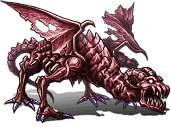
\includegraphics[width=0.31\columnwidth]{./art/monsters/zombiedragon.jpg}}
{
	PV: & \hfill 115 & PM: & \hfill 90\\
	FOR: & \hfill 7 & DEF: & \hfill 5 \\
	MAG: & \hfill 0 & RES: & \hfill 3 \\
	AGI: & \hfill 2 & Tamanho: & \hfill G\\
}
{\accf{Mordida}: 2d Dano \hfill \accf{Imune}:\poison\sleep\silence\blind \hfill  \accf{Fraco}:\holy \\ \accf{Auto-Regenerar}}
{
	\mtech{Cegueiraga}{14}{1r}{3u}{5u}{inimigos na área fazem um teste de DC~8 ou ficam Cegos por 3 rodadas.}{\blind}	
	\mtech{Bafo venenoso}{10}{0r}{3u (frontal)}{Você}{Todos na área sofrem 3d de dano e fazem um teste de DC~8 ou ficam Envenenados por 3 rodadas. }{\poison}	
	\mreaction{Renascimento}{Ao sofre KO, faça um teste de DC~7, se bem sucedido, o KO é removido e recupere 50 PV.}	
}
%
\clearpage
%
%%%%%%%%%%%%%%%%%%%%%%%%%%%%%%%L8%%%%%%%%%%%%%%%%%%%%%%%%%%%%%%%%%%%%%%%%%
%
%
\ofmonster{Midgardsormr}{8}{
\includegraphics[width=0.32\columnwidth]{./art/monsters/midgardsormr.jpg}}
{
	PV: & \hfill 160 & PM: & \hfill 150 \\
	FOR: & \hfill 6 & DEF: & \hfill 7 \\
	MAG: & \hfill 0 & RES: & \hfill 5 \\
	AGI: & \hfill 3 & Tamanho: & \hfill G\\
}
{\accf{Cauda}: 3d Dano \hfill \accf{Imune:}\poison\immobile \hfill \accf{Revidar, Auto-Acerto}}
{	
	\mtech{Mordida}{4}{0r}{Único}{2u}{Se acertar um ataque contra o alvo, ele faz um teste de DC 9 ou fica Envenenado por 3 rodadas. }{\poison}		
	\mtech{Constrição}{6}{0r}{Único}{2u}{Se acertar um ataque contra o alvo, ele faz um teste de DC 9 ou fica Imóvel por 3 rodadas.}{\immobile}	
	\mtech{Cavar}{8}{0r}{2u}{5u}{Cave o chão e não seja atingido por inimigos. No iníncio de cada turno, você emerge num local a 5u e causa 4d de dano a todos os inimigos a 2u daquele ponto.}{}
}
%
\vfill
%
\ofmonster{Behemoth}{8}{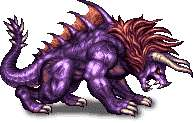
\includegraphics[width=0.31\columnwidth]{./art/monsters/behemoth.jpg}}
{
	PV: & \hfill 220 & PM: & \hfill 160 \\
	FOR: & \hfill 8 & DEF: & \hfill 6 \\
	MAG: & \hfill 6 & RES: & \hfill 5 \\
	AGI: & \hfill 3 & Tamanho: & \hfill G\\
}
{\accf{Garra}: 3d Dano, 2u \hfill \accf{Imune}:\poison\silence \hfill \accf{Resistente:}\fire \\ \accf{Auto-Acelerar, Revidar, Ataque final}}
{
	\mspell{Labareda}{25}{2r}{Único}{7u}{Cause 6d+45 de dano, que ignora RES, ao alvo.}{\fire}	
	\mtech{Içar}{10}{0r}{Único}{2u}{Cause 6d de dano ao alvo e o arremesse no ar a 3u por 1 rodada.}{}		
}
%
\vfill
%
\ofmonster{Ochu}{8}{
\includegraphics[width=0.3\columnwidth]{./art/monsters/ochu.jpg}}
{
	PV: & \hfill 170 & PM: & \hfill 140 \\
	FOR: & \hfill 7 & DEF: & \hfill 6 \\
	MAG: & \hfill 0 & RES: & \hfill 4 \\
	AGI: & \hfill 2 & Tamanho: & \hfill G\\
}
{\accf{Vinhas}: 3d Dano, 3u Alcance \hfill \accf{Resistente:}\water \hfill \accf{Fraco:}\fire \\ \accf{Auto-Regenerar, Golpe duplo} \hfill \accf{Imune}:\poison\sleep\silence\blind}
{	
	\mtech{Semente bala}{8}{0r}{Único}{8u}{O alvo sofre 6d de dano e recebe ReFOR por 1 rodada.}{}	
	\mtech{Pólen}{15}{0r}{3u}{Você}{Inimigos na área fazem um teste de DC 8 e ficam Adormecidos e Envenenados por 3 rodadas.}{\sleep \poison}	
	\mpassive{Vinhas agarradoras}{Alvos que rolem abaixo de 6 no teste de evasão contra seus ataques, ficam Imóveis por 3 rodadas.}
}
%
\newpage
%
\ofmonster{Dragão vermelhon}{8}{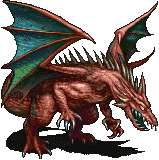
\includegraphics[width=0.24\columnwidth]{./art/monsters/reddragon.jpg}}
{
	PV: & \hfill 180 & PM: & \hfill 140 \\
	FOR: & \hfill 6 & DEF: & \hfill 7 \\
	MAG: & \hfill 5 & RES: & \hfill 5 \\
	AGI: & \hfill 3 & Tamanho: & \hfill G\\
}
{\accf{Mordida}: 3d Dano \hfill \accf{Resistente}:\fire \hfill \accf{Imune}:\sleep\blind\immobile \\ \accf{Revidar, Surto}}
{
	\mspell{Queimar}{12}{0r}{3u (linha)}{Você}{A área é coberta num Campo Ardente por 3 rodadas.}{\fire}	
	\mtech{Chamuscar}{14}{1r}{10u (linha)}{Você}{Cause 6d de dano de Fogo aos inimigos na área.}{\fire}
	\mpassive{Ataque de cauda}{Ao atacar, você pode escolher atingitr os inimigos dentro de 1u de uma vez.}	
}
%
\vfill
%
\ofmonster{Lorde vampiro}{8}{
\includegraphics[width=0.22\columnwidth]{./art/monsters/vampire.jpg}}
{
	PV: & \hfill 160 & PM: & \hfill 200 \\
	FOR: & \hfill 4 & DEF: & \hfill 5 \\
	MAG: & \hfill 8 & RES: & \hfill 6 \\
	AGI: & \hfill 4 & Tamanho: & \hfill M\\
}
{
	\accf{Mordida}: 3d Dano \hfill \accf{Resistente}:\ice\dark\earth \hfill \accf{Fraco}:\fire\holy\\
	\accf{Superimune, Auto-Regenerar}
}
{
	\mspell{Zumbiga}{15}{1r}{Único}{5u}{inimigos na área fazem um teste de DC~8 ou sofrem 4d de dano e ficam Zumbi por 5 rodadas.}{}	
	\mspell{Nevasga}{12}{1r}{Único}{5u}{Cause 6d de dano de Gelo ao alvo.}{\ice}	
	\mspell{Curaga}{14}{1r}{2u}{5u}{Todos na área recuperam 6d de PV.}{}	
	\mtech{Sugar sangue}{8}{0r}{Único}{1u}{Se acertar o ataque contra o alvo, aumente seu PV igual ao mesmo dano causado.}{}
}
%
\vfill
%
%%%%%%%%%%%%%%%%%%%%%%%%%%%%%%%L9%%%%%%%%%%%%%%%%%%%%%%%%%%%%%%%%%%%%%%%%%
%
%
\ofmonster{Tonberry}{9}{
\includegraphics[width=0.28\columnwidth]{./art/monsters/tonberry.jpg}}
{
	PV: & \hfill 240 & PM: & \hfill 0\\
	FOR: & \hfill 15 & DEF: & \hfill 8 \\
	MAG: & \hfill 0 & RES: & \hfill 7 \\
	AGI: & \hfill 2 & Tamanho: & \hfill S\\
}
{\accf{Faca}: 3d Dano \hfill \accf{Imunbe-a-tudo, Reverter}}
{	
	\mpassive{Intimidar}{Ao se mover a 3u de um inimigo, ele faz um teste de DC~8 ou fica Imóvel por 1 rodada.}	
	\mpassive{Rancor}{Ao atacar um inimigo, ele faz um teste de DC 7 ou sofre KO. }	
	\mreaction{Carma}{Sempre que o inimigo está a mais de 3u de você lhe causa dano, cause 6d de dano de Escuridão a ele. }
}
%
\clearpage
%
\ofmonster{Kraken}{9}{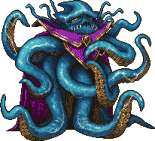
\includegraphics[width=0.25\columnwidth]{./art/monsters/kraken.jpg}}
{
	PV: & \hfill 250 & PM: & \hfill 300 \\
	FOR: & \hfill 8 & DEF: & \hfill 6 \\
	MAG: & \hfill 10 & RES: & \hfill 7 \\
	AGI: & \hfill 2 & Tamanho: & \hfill G\\
}
{
	\accf{Tentáculo}: 3d Dano, 2u Alcance\hfill \accf{Resistente}:\water\ice\\
	\accf{Auto-Acelerar, Revidar, Golpe duplo} \hfill \accf{Imune}:\poison\sleep 
}
{	
	\mspell{Águaga}{14}{1r}{Único}{6u}{cause 6d de dano de Água ao alvo. }{\water}	
	\mtech{Tinta}{15}{1r}{3u}{6u}{Inimigos na área fazem um teste de DC 8 ou ficam Cegos e sofrem 4d de dano.}{\blind}
	\mtech{Inundação}{18}{1r}{100u}{Você}{Todos na área, exceto você, sofrem 4d de dano de Água. Além disso, a área é coberta num Campo Vagaroso por 3 rodadas, que não o afeta.}{}
}
%
\vfill
%
\ofmonster{Adamantoise}{9}{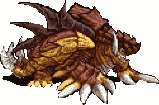
\includegraphics[width=0.32\columnwidth]{./art/monsters/adamantoise.jpg}}
{
	PV: & \hfill 300 & PM: & \hfill 250 \\
	FOR: & \hfill 8 & DEF: & \hfill 7 \\
	MAG: & \hfill 6 & RES: & \hfill 6 \\
	AGI: & \hfill 1 & Tamanho: & \hfill G\\
}
{
	\accf{Atropelar}: 3d Dano, 2u Alvo \hfill \accf{Imune}:\poison\silence \\
	\accf{Auto-Regenerar, Ataque final, Surto} \hfill \accf{Resistente}:\earth
}
{	
	\mspell{Última}{28}{2r}{2u}{7u}{CAuse 6d+30 de dano de Escuridão aos inimigos na área.}{\dark}	
	\mtech{Rugido}{15}{0r}{5u}{Você}{Inimigos dentro da área fazem um teste de DC 8 ou ficam Imóveis por 3 rodadas. }{\immobile}	
}
%
\vfill
%
\ofmonster{Lich}{9}{
\includegraphics[width=0.28\columnwidth]{./art/monsters/lich.jpg}}
{
	PV: & \hfill 250 & PM: & \hfill 300\\
	FOR: & \hfill 5 & DEF: & \hfill 6 \\
	MAG: & \hfill 12 & RES: & \hfill 8 \\
	AGI: & \hfill 2 & Tamanho: & \hfill G\\
}
{
	\accf{Raio de energia}: 3d Dano, 5u Alcance\hfill \accf{Resistente}:\dark \\
	\accf{Superimune, Auto-Regenerar, Auto-Acelerar}  
}
{	
	\mspell{Zumbiga}{15}{1r}{Único}{5u}{Inimigos na área fazem um teste de DC~8 ou sofrem 4d de dano e ficam Zumbi por 5 rodadas.}{}	
	\mspell{Envenenaga}{18}{1r}{3u}{5u}{Todos na área fazem um teste de DC 8 ou ficam Envenenados por 3 rodadas.}{\poison}	
	\mspell{Perdição}{18}{0r}{Único}{5u}{O alvo faz um teste de DC 8  ou sofre KO após 3 rodadas.}{\ko}	
}
%
\newpage
%
\ofmonster{Visão da morte}{9}{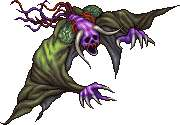
\includegraphics[width=0.3\columnwidth]{./art/monsters/deathgaze.jpg}}
{
	PV: & \hfill 230 & PM: & \hfill 350 \\
	FOR: & \hfill 7 & DEF: & \hfill 6 \\
	MAG: & \hfill 11 & RES: & \hfill 8 \\
	AGI: & \hfill 4 & Tamanho: & \hfill G\\
}
{
	\accf{Garra}: 3d Dano, 2u Alcance \hfill \accf{Resistente}:\ice \hfill \accf{Fraci:}\holy \\
	\accf{Superimune, Auto-Oscilar, Auto-Acelerar}
}
{	
	\mspell{Mega-Perdição}{30}{1r}{3u}{5u}{
		Inimigos na área fazem um teste de DC~8 ou sofrem KO após 3 rodadas.
	}{\ko}
	\mspell{Nevasga}{12}{1r}{Único}{5u}{Cause 6d de dano de Gelo ao alvo.}{\ice}		
	\mtech{Recuar}{0}{0r}{Único}{Self}{Faça um teste de DC~7 e se bem sucedido, remova-se da batalha de imediato.}{}				
	%\mpassive{Deathtouch}{Whenever you successfully Attack a target, he makes a DC 6 check and immediately suffers KO upon failure.}
	\mreaction{Auto-Dissipar}{Sempre que um inimigo denrto de 5u de você, recebe um Efeito de estado benéfico, você pode fazer um teste de DC 7. Se bem sucedido, o efeito sobre o alvo é removido de imediato.}	
}
%
\vfill
%
%%%%%%%%%%%%%%%%%%%%%%%%%%%%%%%L9%%%%%%%%%%%%%%%%%%%%%%%%%%%%%%%%%%%%%%%%%
%
\ofmonster{Ozma}{10}{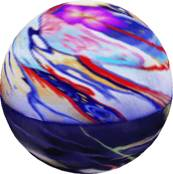
\includegraphics[width=0.23\columnwidth]{./art/monsters/ozma.jpg}}
{
	PV: & \hfill 300 & PM: & \hfill 400 \\
	FOR: & \hfill 4 & DEF: & \hfill 5 \\
	MAG: & \hfill 12 & RES: & \hfill 8 \\
	AGI: & \hfill 2 & Tamanho: & \hfill G\\
}
{
	\accf{Feixe}: 4d Dano, 8u Alcance \hfill \accf{Resistente}:\fire\ice\lightning\earth \\
	\accf{Superimune, Auto-Acelerar, Retaliar, TC-0}
}
{
	\mspell{Curaga}{14}{0r}{2u}{5u}{Aliados na área recuperam 6d de PV.}{}
	\mspell{Raiaja}{18}{0r}{2u}{8u}{Todos na área sofrem 6d+15 de dano de Raio.}{\lightning}		
	\mspell{Juizo final}{20}{0r}{2u}{10u}{Inimigos na área fazem um teste de DC~6 ou sofrem KO ou 6d de dano se bem sucedidos.}{\earth}				
	\mspell{Maldição}{16}{0r}{Único}{5u}{O alvo faz um teste de DC~8 ou fica Envenenado, Mudo e Imóvel.}{}	
	\mspell{Absorver PM}{0}{0r}{Único}{10u}{Reduza o PM do alvo em 4d e aumente o seu na mesma quantidade.}{}	
	\mreaction{Revidar Turbo}{Sempre que sofrer dano de um inimigo, faça um teste de DC~8. Se bem sucedido, tenha um turno extra imediatamnte ao agressor.}
}
%
\clearpage
%
\ofmonster{Arma Rubi}{10}{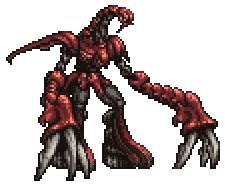
\includegraphics[width=0.3\columnwidth]{./art/monsters/rubyweapon.jpg}}
{
	PV: & \hfill 400 & PM: & \hfill 300 \\
	FOR: & \hfill 12 & DEF: & \hfill 9 \\
	MAG: & \hfill 6 & RES: & \hfill 7 \\
	AGI: & \hfill 2 & Tamanho: & \hfill G\\
}
{
	\accf{Raio de energia rubi}: 4d Dano, 10u Alcance \\ \accf{Resistente}:\earth\dark \\
	\accf{Superimune, Auto-Regenerar, Revidar, Surto} 
}
{
	\mtech{Redemoinho de areia}{10}{1r}{10u (linha)}{Você}{Todos na área são empurrados até 10u e ficam Cegos e sofrem 6d+10 de dano de Terra. }{\earth}				
	\mspell{Chama rubi}{12}{1r}{Único}{8u}{O alvo sofre 6d+15 de dano de Fogo, não reduzido por RES.}{\dark}
	\mspell{Cometa}{18}{1r}{5u}{10u}{Todos na área sofrem 6d+10 de dano e recebem ReDEF por 3 rodadas.}{\dark}
	\mtech{Tentáculos enterrados}{8}{0r}{1u}{10u}{Enterre seus braços no chão e 2 tentáculos de 1u de tamanho surgem do chão num local dentro do alcance, causando 8d de dano a todos dentro da área deles. 
	Enquanto estiverem enterrados, você não pode se mover e precisa usar uma ação para desenterrá-los. Enquanto isso, cada um deles pode atacar (4d Dano) contra inimigos que estejam a 3u deles além de sua ação normal a cada turno.
}{}	
}
%
\vfill
%
\ofmonster{Caos}{10}{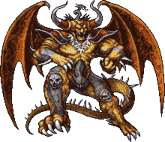
\includegraphics[width=0.26\columnwidth]{./art/monsters/chaos.jpg}}
{
	PV: & \hfill 400 & PM: & \hfill 400 \\
	FOR: & \hfill 9 & DEF: & \hfill 7 \\
	MAG: & \hfill 11 & RES: & \hfill 8 \\
	AGI: & \hfill 3 & Tamanho: & \hfill G\\
}
{
	\accf{Feixe}: 4d Dano, 5u Alcanc\hfill \accf{Resistente}:\dark\fire \\
	\accf{Superimune, Auto-Acelerar, Retaliar, Reverter, Surto}  
}
{	
	\mspell{Zona-X}{13}{0r}{3u}{8u}{Crie um Campo de efeito de sua escolha na área por 3 rodadas.}{}		
	\mspell{Última}{30}{2r}{50u}{Você}{Cause 6d+40 de dano de Escuridão aos inimigos na área.}{\dark}	
	\mspell{Curaja}{20}{1r}{2u}{8u}{Aliados na área recuperam 6d+15 de PV. }{}	
	\mspell{Fogaja}{18}{1r}{2u}{8u}{Cause 6d+15 de dano de Fogo a todos na área. }{\fire}
	\mpassive{Toque do Caos}{Todos que rolarem abaixo de 6 no teste de evasão contra seus ataques, ficam Cegos e Mudos por 3 rodadas.}
}
%
\newpage
%
\ofmonster{Shinryu}{10}{\includegraphics[width=0.2\columnwidth]{./art/monsters/shinryu.jpg}}
{
	PV: & \hfill 500 & PM: & \hfill 500 \\
	FOR: & \hfill 12 & DEF: & \hfill 9 \\
	MAG: & \hfill 14 & RES: & \hfill 9 \\
	AGI: & \hfill 3 & Tamanho: & \hfill G\\
}
{
	\accf{Cauda}: 4d Dano, 4u Alcance \\
	\accf{Imuna-a-tudo, Auto-Acelerar, Auto-Regenerar, Revidar, Retaliar}
}
{
	\mspell{Nevasja}{18}{1r}{2u}{8u}{Todos na área sofrem 6d+15 de dano de Gelo.}{\ice}		
	\mspell{Maremoto}{22}{1r}{10u (frontal)}{Você}{Inimigos na área sofrem 6d+10 de dano de Água e ficam Imóveis por 2 rodadas.}{\water \immobile}	
	\mspell{Raios Atômicos}{20}{1r}{8u}{Você}{Inimigos na área sofrem 6d de dano de Fogo e ficam Envenenados por 3 rodadas.}{\fire \poison}		
	\mpassive{Adaptar-se ao elemento}{
		No início de cada turno, escolha um elemento (ex.: fogo). Ganhe Resistência a ele até o início de seu próximo turno.
	}
}
%
\vfill
%
\ofmonster{Ômega}{???}{\includegraphics[width=0.3\columnwidth]{./art/monsters/omega.jpg}}
{
	PV: & \hfill 999 & PM: & \hfill 999 \\
	FOR: & \hfill 19 & DEF: & \hfill 11 \\
	MAG: & \hfill 17 & RES: & \hfill 10 \\
	AGI: & \hfill 4 & Tamanho: & \hfill G\\
}
{
	\accf{Lazer}: 4d Dano, 10u Alcance\hfill \accf{Resistente}:\fire\dark\lightning \\
	\accf{Superimune, Auto-Oscilar, Auto-Acelerar, Auto-Regenerar, Revidar, Golpe duplo, Reverter, Retaliar, Surto}
}
{	
	\mspell{Derreter}{30}{1r}{10u}{Você}{Uma vulnerabilidade do sistema o força a vazar memória sigilosa e lava. CAuse 6d+40 de dano de Fogo ao alvo, incluindo a si mesmo. }{\fire}	
	\mtech{Risco biológico}{16}{0r}{3u}{10u}{Inimigos na área fazem um teste de DC~8 e ficam Envenenados, Cegos e Lentos por 3 rodadas.}{\fire}
	\mtech{Lança-chamas}{8}{0r}{3u (frontal)}{Você}{Cause 6d+10 de dano de Fogo aos inimigos na área. Além disso, a área também é cobertar num Campo Ardente por 3 rodadas.}{\fire}
	\mtech{Canhão de onda}{14}{1r}{3u}{12u}{Cause 6d+20 de dano de Escuridão e imponha ReDEF, ReRES e ReFOR por 5 rodadas a todos na área. }{\dark \dedef \deres}		\\
	\vspace*{-0.2cm}\\
	\ofquote{”O homem forja uma arma para destruir os deuses: Ômega. Ela não conhece compaixão, apenas destruição! Não há comparação à sua força. O sábio não se atreve a cruzar o seu caminho, receosos de encontrarem o seu fim."}{Gentiana}
}
%
%
\clearpage